\documentclass[a4paper,11pt]{exam}
\usepackage[utf8]{inputenc}
%\usepackage{lipsum}
\usepackage[]{algorithm2e}

\date{\today}
\title{UFR 27 --- L2 MIASHS Renforcement Informatique \\ {Développement WEB} \\  \normalsize{Durée de l'épreuve: 1h30} } 
\author{Responsable: Nicolas Herbaut}
\date{16 Janvier 2019}

\usepackage{pdfpages}
\usepackage{listings}
\usepackage{graphicx}
\usepackage{textcomp}
\usepackage{multicol}


\setlength{\columnseprule}{1pt}
\def\columnseprulecolor{\color{black}}

\rhead{L2 MIASHS --- Université Paris 1 Panthéon Sorbonne}
\lhead{Introduction au développement WEB}

\ifdefined\issolution
\printanswers
\fi

\usepackage{inconsolata}
\usepackage{listings}
\usepackage{color}

\definecolor{pblue}{rgb}{0.13,0.13,1}
\definecolor{pgreen}{rgb}{0,0.5,0}
\definecolor{pred}{rgb}{0.9,0,0}
\definecolor{pgrey}{rgb}{0.46,0.45,0.48}

\lstset{language=sh,basicstyle=\ttfamily,columns=fullflexible}


\lstset{inputencoding=latin1}

\lstset{language=Java,
  showspaces=false,
  showtabs=false,
  breaklines=true,
  showstringspaces=false,
  breakatwhitespace=true,
  commentstyle=\color{pgreen},
  keywordstyle=\color{pblue},
  stringstyle=\color{pred},
  basicstyle=\ttfamily,
  moredelim=[il][\textcolor{pgrey}]{$ $},
  moredelim=[is][\textcolor{pgrey}]{\%\%}{\%\%}
}

\lstdefinelanguage{CSS}{
  morekeywords={accelerator,azimuth,background,background-attachment,
    background-color,background-image,background-position,
    background-position-x,background-position-y,background-repeat,
    behavior,border,border-bottom,border-bottom-color,
    border-bottom-style,border-bottom-width,border-collapse,
    border-color,border-left,border-left-color,border-left-style,
    border-left-width,border-right,border-right-color,
    border-right-style,border-right-width,border-spacing,
    border-style,border-top,border-top-color,border-top-style,
    border-top-width,border-width,bottom,caption-side,clear,
    clip,color,content,counter-increment,counter-reset,cue,
    cue-after,cue-before,cursor,direction,display,elevation,
    empty-cells,filter,float,font,font-family,font-size,
    font-size-adjust,font-stretch,font-style,font-variant,
    font-weight,height,ime-mode,include-source,
    layer-background-color,layer-background-image,layout-flow,
    layout-grid,layout-grid-char,layout-grid-char-spacing,
    layout-grid-line,layout-grid-mode,layout-grid-type,left,
    letter-spacing,line-break,line-height,list-style,
    list-style-image,list-style-position,list-style-type,margin,
    margin-bottom,margin-left,margin-right,margin-top,
    marker-offset,marks,max-height,max-width,min-height,
    min-width,-moz-binding,-moz-border-radius,
    -moz-border-radius-topleft,-moz-border-radius-topright,
    -moz-border-radius-bottomright,-moz-border-radius-bottomleft,
    -moz-border-top-colors,-moz-border-right-colors,
    -moz-border-bottom-colors,-moz-border-left-colors,-moz-opacity,
    -moz-outline,-moz-outline-color,-moz-outline-style,
    -moz-outline-width,-moz-user-focus,-moz-user-input,
    -moz-user-modify,-moz-user-select,orphans,outline,
    outline-color,outline-style,outline-width,overflow,
    overflow-X,overflow-Y,padding,padding-bottom,padding-left,
    padding-right,padding-top,page,page-break-after,
    page-break-before,page-break-inside,pause,pause-after,
    pause-before,pitch,pitch-range,play-during,position,quotes,
    -replace,richness,right,ruby-align,ruby-overhang,
    ruby-position,-set-link-source,size,speak,speak-header,
    speak-numeral,speak-punctuation,speech-rate,stress,
    scrollbar-arrow-color,scrollbar-base-color,
    scrollbar-dark-shadow-color,scrollbar-face-color,
    scrollbar-highlight-color,scrollbar-shadow-color,
    scrollbar-3d-light-color,scrollbar-track-color,table-layout,
    text-align,text-align-last,text-decoration,text-indent,
    text-justify,text-overflow,text-shadow,text-transform,
    text-autospace,text-kashida-space,text-underline-position,top,
    unicode-bidi,-use-link-source,vertical-align,visibility,
    voice-family,volume,white-space,widows,width,word-break,
    word-spacing,word-wrap,writing-mode,z-index,zoom},
  morestring=[s]{:}{;},
  sensitive,
  morecomment=[s]{/*}{*/}
}

\lstset{
     literate=%
         {á}{{\'a}}1
         {í}{{\'i}}1
		 {é}{{\'e}}1
		 {ê}{{\^e}}1
		 {à}{{\`a }}1
		 {è}{{\`e}}1
         {ý}{{\'y}}1
		 {ú}{{\'u}}1
		 {î}{{\^i}}1
		 {ù}{{\`u}}1
		 {ó}{{\'o}}1
		 {ô}{{\^o}}1
         {ě}{{\v{e}}}1
         {š}{{\v{s}}}1
         {č}{{\v{c}}}1
         {ř}{{\v{r}}}1
         {ž}{{\v{z}}}1
         {ď}{{\v{d}}}1
         {ť}{{\v{t}}}1
         {ň}{{\v{n}}}1                
         {ů}{{\r{u}}}1
         {Á}{{\'A}}1
         {Í}{{\'I}}1
         {É}{{\'E}}1
         {Ý}{{\'Y}}1
         {Ú}{{\'U}}1
         {Ó}{{\'O}}1
         {Ě}{{\v{E}}}1
         {Š}{{\v{S}}}1
         {Č}{{\v{C}}}1
         {Ř}{{\v{R}}}1
         {Ž}{{\v{Z}}}1
         {Ď}{{\v{D}}}1
         {Ť}{{\v{T}}}1
         {Ň}{{\v{N}}}1                
         {Ů}{{\r{U}}}1    
}

\lstdefinelanguage{JavaScript}{
  keywords={typeof, new, true, false, catch, function, return, null, catch, switch, var, if, in, while, do, else, case, break},
  keywordstyle=\color{blue}\bfseries,
  ndkeywords={class, export, boolean, throw, implements, import, this},
  ndkeywordstyle=\color{darkgray}\bfseries,
  identifierstyle=\color{black},
  sensitive=false,
  comment=[l]{//},
  morecomment=[s]{/*}{*/},
  commentstyle=\color{purple}\ttfamily,
  stringstyle=\color{red}\ttfamily,
  morestring=[b]',
  morestring=[b]"
}

\lstset{
   language=JavaScript,
   backgroundcolor=\color{lightgray},
   extendedchars=true,
   basicstyle=\footnotesize\ttfamily,
   showstringspaces=false,
   showspaces=false,
   numbers=left,
   numberstyle=\footnotesize,
   numbersep=9pt,
   tabsize=2,
   breaklines=true,
   showtabs=false,
   captionpos=b
}



\begin{document}
\maketitle

\noindent N° carte d'étudiant :  \fillin \\ \\


\noindent \textbf{Aucun document n'est autorisé. Un aide mémoire a été ajouté à la fin du sujet.\\
\noindent Vous devez répondre aux parties 1 et 2 directement sur le sujet, pensez donc à remettre ce sujet à l'intérieur de votre copie d'examen !\\
\noindent Les téléphones et autres mobiles/tablettes doivent être éteints dans votre sac. Le sac doit être posé au sol devant le tableau
}








\section{Bases des languages (3 pts)}

\begin{questions}

	\question[1] Que signifie CSS?
	\begin{solutionorlines}[3cm]
		Cascading Stylesheets
	\end{solutionorlines}

	\question[1] Quel est le rôle du HTML dans une page WEB?
	\begin{solutionorlines}[3cm]
		Le HTML permet de structurer les données affichées dans une page web. Il est responsable de l'expression du contenu.
		
	\end{solutionorlines}

	\question[1] Quelle balise est utilisée pour créer des liens dans une page web? Donnez un exemple d'un lien vers le site de votre Université.
	\begin{solutionorlines}[3cm]
		\begin{lstlisting}[frame=leftline,language={HTML},numbers=none]  
<a href="https://pantheonsorbonne.fr">Mon université</a>
		\end{lstlisting}
	\end{solutionorlines}

\end{questions}

\section{Mise en page simple (5pt)}
On souhaite obtenir le rendu suivant pour la page principal d'un site.

\begin{center}
\fbox{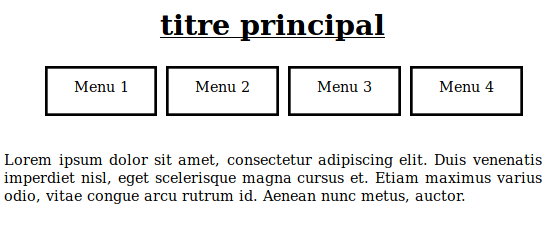
\includegraphics[width=0.5\textwidth]{exo1.png}}
\end{center}

\begin{questions}
	\question[2.5] Donnez le HTML cor
	respondant à ce qui est affiché. Pour cela, vous utiliserez des listes non ordonnées pour les menus.
	\begin{solutionorlines}[5cm]
		\scriptsize
		\begin{lstlisting}[frame=leftline,language={HTML},numbers=none]  
<div id="title"><h1>titre principal</h1>
  <ul>
    <li>Menu 1</li>
    <li>Menu 2</li>
    <li>Menu 3</li>
    <li>Menu 4</li>
  </ul>
<p>Lorem ipsum dolor sit amet, consectetur adipiscing elit. Duis venenatis imperdiet nisl, eget scelerisque magna cursus et. Etiam maximus varius odio, vitae congue arcu rutrum id. Aenean nunc metus, auctor. </p>
</div>
\end{lstlisting}


	\end{solutionorlines}
  \question[2.5] Donnez le CSS correspondant à ce qui est affiché. Pour cela, nous vous donnons les spécifications supplémentaires suivantes:
  \scriptsize
	\begin{itemize}
		\item tout le contenu doit être centré horizontalement sur la page, avec une largeur de 600px et une hauteur de 100px
		\item le titre principal doit être souligné et centré horizontalement
		\item le paragraphe doit être justifié
		\item chaque élément du menu doit mesurer 30x100 px
		\item avoir un margin de 5px et un padding de 10px
		\item chaque élément du menu doit avoir une bordure
		\item chaque élément du menu doit être flottant et centré
		\item le menu en lui même doit être séparé du paragraphe de 30px et sa hauteur totale doit être de 70px
  \end{itemize}
  \begin{multicols}{3}
  \begin{solutionorlines}[6.8cm]
		\scriptsize
		\begin{lstlisting}[frame=leftline,language={CSS},numbers=none]  
div{
  width:600px;
  margin:auto;
  height:100px;
}
h1{
  text-decoration:underline;
  text-align:center;
}

p{
  text-align:justify;
}
li{
  height:30px;
  float:left;
  list-style:none;
  width:100px;
  text-align:center;
  border-style:solid;
  padding:10px;
  margin:5px;
}
ul{
  margin-bottom:30px;
  height:70px;
}
		\end{lstlisting}
  \end{solutionorlines}
  \begin{solutionorlines}[6.8cm]
  \end{solutionorlines}
  \begin{solutionorlines}[6.7cm]
  \end{solutionorlines}
\end{multicols}

\end{questions}


 \section{Mini-calculatrice JavaScript}

 On souhaite réaliser une mini-calculatrice en JS qui est exécutée par le navigateur.
 \begin{center}
	\fbox{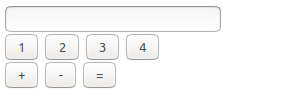
\includegraphics[width=0.5\textwidth]{calc.png}}
	\end{center}
 Voici un exemple de séquence d'appel:
 \begin{enumerate}
	\scriptsize \itemsep0em 
	\item clic sur 1 
	\item l'élément total affiche 1
	\item clic sur 2
	\item l'élément total affiche 12
	\item clic sur +
	\item l'élément total est vidé
	\item click sur 3
	\item l'élément total affiche 3
	\item click sur "="
	\item l'élément total affiche 15.
 \end{enumerate}
 

	\begin{questions}

		\question[4] Donnez le HTML permettant d'afficher cette mini-calculatrice. Vous prendrez bien soin de donner des classes aux éléments remplissant la même fonction (nombres, opérateurs...) et des id aux éléments remplissant une fonction unique (égal, total...)
		\begin{solutionorlines}[0cm]
			\begin{lstlisting}[frame=leftline,language={HTML},numbers=none]  
<input id="total">
<br>
<input class="number" id="btn1" type="button" value="1"/>
<input class="number" id="btn2" type="button" value="2"/>
<input class="number" id="btn3" type="button" value="3"/>
<input class="number" id="btn4" type="button" value="4"/>
<br>
<input class="operator" type="button" value="+"/>
<input class="operator" type="button" value="-"/>
<input id="equals" type="button" value="="/>
		    \end{lstlisting}
		\end{solutionorlines}
		\question[4] Donnez le code JS permettant d'enregistrer les évènements  sur les boutons. On rappelle que la fonction que vous devez créer pour recevoir le déclenchement d'un évènement (ici "event") est de la forme:
		\begin{lstlisting}[frame=leftline,language={JavaScript},numbers=none]  

//elt=l'élément sur lequel enregistrer l'évènement
elt.addEventListener("event",callback);

//la fonction qui va traiter l'évènement
function callback(evt){
 var value = evt.target.value;
 //ici la variable value permet d'accéder à la valeur de l'élément cliqué,
 //passé en paramètre de la fonction
}
		\end{lstlisting}
		\begin{solutionorlines}[0cm]
			\begin{lstlisting}[frame=leftline,language={JavaScript},numbers=none]  
for(let btn of document.getElementsByClassName("number")){
	btn.addEventListener("click",handleButton);
};
for(let op of document.getElementsByClassName("operator")){
	op.addEventListener("click",handleOperator);
}
document.getElementById("equals").addEventListener("click",handleEquals);
		    \end{lstlisting}
		\end{solutionorlines}

		\question[4] Donnez le code permettant de faire fonctionner la calculatrice.
		\begin{solutionorlines}[0cm]
			\begin{lstlisting}[frame=leftline,language={JavaScript},numbers=none]  
var operand1=0;
var operator="";
for(let btn of document.getElementsByClassName("number")){
btn.addEventListener("click",handleNumber);
};

for(let op of document.getElementsByClassName("operator")){
	op.addEventListener("click",handleOperator);
};
document.getElementById("equals").addEventListener("click",handleEquals);

function handleNumber(evt){
	document.getElementById("total").value+=evt.target.value;
}
function handleOperator(evt){
	operator=evt.target.value;
	operand1=parseInt(document.getElementById("total").value);
	document.getElementById("total").value="";
};

function handleEquals(evt){
	computeOperation();
};

function computeOperation(){
	var value=0;
	if(operator=="+"){
	value=operand1+parseInt(document.getElementById("total").value);
	}
	else{
	value=operand1-parseInt(document.getElementById("total").value);
	}
	document.getElementById("total").value=value;
}
		    \end{lstlisting}
		\end{solutionorlines}

	\end{questions}

\newpage
\includepdf[pages=-,fitpaper=true,scale=0.8,]{../../cheatsheets/js.pdf}
\includepdf[pages=-,fitpaper=true,scale=0.8,]{../../cheatsheets/css.pdf}
\includepdf[pages=-,fitpaper=true,scale=0.8,]{../../cheatsheets/html.pdf}

\end{document}
